\PassOptionsToPackage{unicode=true}{hyperref} % options for packages loaded elsewhere
\PassOptionsToPackage{hyphens}{url}
%
\documentclass[]{article}
\usepackage{lmodern}
\usepackage{amssymb,amsmath}
\usepackage{ifxetex,ifluatex}
\usepackage{fixltx2e} % provides \textsubscript
\ifnum 0\ifxetex 1\fi\ifluatex 1\fi=0 % if pdftex
  \usepackage[T1]{fontenc}
  \usepackage[utf8]{inputenc}
  \usepackage{textcomp} % provides euro and other symbols
\else % if luatex or xelatex
  \usepackage{unicode-math}
  \defaultfontfeatures{Ligatures=TeX,Scale=MatchLowercase}
\fi
% use upquote if available, for straight quotes in verbatim environments
\IfFileExists{upquote.sty}{\usepackage{upquote}}{}
% use microtype if available
\IfFileExists{microtype.sty}{%
\usepackage[]{microtype}
\UseMicrotypeSet[protrusion]{basicmath} % disable protrusion for tt fonts
}{}
\IfFileExists{parskip.sty}{%
\usepackage{parskip}
}{% else
\setlength{\parindent}{0pt}
\setlength{\parskip}{6pt plus 2pt minus 1pt}
}
\usepackage{hyperref}
\hypersetup{
            pdftitle={Métodos Quantitativos},
            pdfauthor={Prof.~Dr.~A. L. Korzenowski},
            pdfborder={0 0 0},
            breaklinks=true}
\urlstyle{same}  % don't use monospace font for urls
\usepackage[margin=1in]{geometry}
\usepackage{color}
\usepackage{fancyvrb}
\newcommand{\VerbBar}{|}
\newcommand{\VERB}{\Verb[commandchars=\\\{\}]}
\DefineVerbatimEnvironment{Highlighting}{Verbatim}{commandchars=\\\{\}}
% Add ',fontsize=\small' for more characters per line
\usepackage{framed}
\definecolor{shadecolor}{RGB}{248,248,248}
\newenvironment{Shaded}{\begin{snugshade}}{\end{snugshade}}
\newcommand{\AlertTok}[1]{\textcolor[rgb]{0.94,0.16,0.16}{#1}}
\newcommand{\AnnotationTok}[1]{\textcolor[rgb]{0.56,0.35,0.01}{\textbf{\textit{#1}}}}
\newcommand{\AttributeTok}[1]{\textcolor[rgb]{0.77,0.63,0.00}{#1}}
\newcommand{\BaseNTok}[1]{\textcolor[rgb]{0.00,0.00,0.81}{#1}}
\newcommand{\BuiltInTok}[1]{#1}
\newcommand{\CharTok}[1]{\textcolor[rgb]{0.31,0.60,0.02}{#1}}
\newcommand{\CommentTok}[1]{\textcolor[rgb]{0.56,0.35,0.01}{\textit{#1}}}
\newcommand{\CommentVarTok}[1]{\textcolor[rgb]{0.56,0.35,0.01}{\textbf{\textit{#1}}}}
\newcommand{\ConstantTok}[1]{\textcolor[rgb]{0.00,0.00,0.00}{#1}}
\newcommand{\ControlFlowTok}[1]{\textcolor[rgb]{0.13,0.29,0.53}{\textbf{#1}}}
\newcommand{\DataTypeTok}[1]{\textcolor[rgb]{0.13,0.29,0.53}{#1}}
\newcommand{\DecValTok}[1]{\textcolor[rgb]{0.00,0.00,0.81}{#1}}
\newcommand{\DocumentationTok}[1]{\textcolor[rgb]{0.56,0.35,0.01}{\textbf{\textit{#1}}}}
\newcommand{\ErrorTok}[1]{\textcolor[rgb]{0.64,0.00,0.00}{\textbf{#1}}}
\newcommand{\ExtensionTok}[1]{#1}
\newcommand{\FloatTok}[1]{\textcolor[rgb]{0.00,0.00,0.81}{#1}}
\newcommand{\FunctionTok}[1]{\textcolor[rgb]{0.00,0.00,0.00}{#1}}
\newcommand{\ImportTok}[1]{#1}
\newcommand{\InformationTok}[1]{\textcolor[rgb]{0.56,0.35,0.01}{\textbf{\textit{#1}}}}
\newcommand{\KeywordTok}[1]{\textcolor[rgb]{0.13,0.29,0.53}{\textbf{#1}}}
\newcommand{\NormalTok}[1]{#1}
\newcommand{\OperatorTok}[1]{\textcolor[rgb]{0.81,0.36,0.00}{\textbf{#1}}}
\newcommand{\OtherTok}[1]{\textcolor[rgb]{0.56,0.35,0.01}{#1}}
\newcommand{\PreprocessorTok}[1]{\textcolor[rgb]{0.56,0.35,0.01}{\textit{#1}}}
\newcommand{\RegionMarkerTok}[1]{#1}
\newcommand{\SpecialCharTok}[1]{\textcolor[rgb]{0.00,0.00,0.00}{#1}}
\newcommand{\SpecialStringTok}[1]{\textcolor[rgb]{0.31,0.60,0.02}{#1}}
\newcommand{\StringTok}[1]{\textcolor[rgb]{0.31,0.60,0.02}{#1}}
\newcommand{\VariableTok}[1]{\textcolor[rgb]{0.00,0.00,0.00}{#1}}
\newcommand{\VerbatimStringTok}[1]{\textcolor[rgb]{0.31,0.60,0.02}{#1}}
\newcommand{\WarningTok}[1]{\textcolor[rgb]{0.56,0.35,0.01}{\textbf{\textit{#1}}}}
\usepackage{graphicx,grffile}
\makeatletter
\def\maxwidth{\ifdim\Gin@nat@width>\linewidth\linewidth\else\Gin@nat@width\fi}
\def\maxheight{\ifdim\Gin@nat@height>\textheight\textheight\else\Gin@nat@height\fi}
\makeatother
% Scale images if necessary, so that they will not overflow the page
% margins by default, and it is still possible to overwrite the defaults
% using explicit options in \includegraphics[width, height, ...]{}
\setkeys{Gin}{width=\maxwidth,height=\maxheight,keepaspectratio}
\setlength{\emergencystretch}{3em}  % prevent overfull lines
\providecommand{\tightlist}{%
  \setlength{\itemsep}{0pt}\setlength{\parskip}{0pt}}
\setcounter{secnumdepth}{0}
% Redefines (sub)paragraphs to behave more like sections
\ifx\paragraph\undefined\else
\let\oldparagraph\paragraph
\renewcommand{\paragraph}[1]{\oldparagraph{#1}\mbox{}}
\fi
\ifx\subparagraph\undefined\else
\let\oldsubparagraph\subparagraph
\renewcommand{\subparagraph}[1]{\oldsubparagraph{#1}\mbox{}}
\fi

% set default figure placement to htbp
\makeatletter
\def\fps@figure{htbp}
\makeatother

\usepackage{etoolbox}
\makeatletter
\providecommand{\subtitle}[1]{% add subtitle to \maketitle
  \apptocmd{\@title}{\par {\large #1 \par}}{}{}
}
\makeatother
% https://github.com/rstudio/rmarkdown/issues/337
\let\rmarkdownfootnote\footnote%
\def\footnote{\protect\rmarkdownfootnote}

% https://github.com/rstudio/rmarkdown/pull/252
\usepackage{titling}
\setlength{\droptitle}{-2em}

\pretitle{\vspace{\droptitle}\centering\huge}
\posttitle{\par}

\preauthor{\centering\large\emph}
\postauthor{\par}

\predate{\centering\large\emph}
\postdate{\par}

\title{Métodos Quantitativos}
\author{Prof.~Dr.~A. L. Korzenowski}
\date{}

\begin{document}
\maketitle

\hypertarget{aula-03-modelos-lineares-de-regressuxe3o-e-generalizados}{%
\section{Aula 03: Modelos Lineares de Regressão e
Generalizados}\label{aula-03-modelos-lineares-de-regressuxe3o-e-generalizados}}

\hypertarget{multiple-linear-regression}{%
\subsection{Multiple (Linear)
Regression}\label{multiple-linear-regression}}

A regressão linear simples é utilizada para analisar relações entre
variáveis contínuas. Para fazer a regressão no R a função é
\textbf{lm()}, para linear models. A seguir temos um exemplo de
aplicação das funções e discutiremos os conceitos em conjunto com os
resultados.

\begin{Shaded}
\begin{Highlighting}[]
\CommentTok{# Multiple Linear Regression Example }
\KeywordTok{require}\NormalTok{(car)}
\KeywordTok{attach}\NormalTok{(mtcars)}
\NormalTok{fit <-}\StringTok{ }\KeywordTok{lm}\NormalTok{(mpg }\OperatorTok{~}\StringTok{ }\NormalTok{hp }\OperatorTok{+}\StringTok{ }\NormalTok{wt }\OperatorTok{+}\StringTok{ }\NormalTok{vs, }\DataTypeTok{data=}\NormalTok{mtcars)}
\KeywordTok{summary}\NormalTok{(fit) }\CommentTok{# show results}
\end{Highlighting}
\end{Shaded}

\begin{verbatim}
## 
## Call:
## lm(formula = mpg ~ hp + wt + vs, data = mtcars)
## 
## Residuals:
##     Min      1Q  Median      3Q     Max 
## -3.4667 -1.4857 -0.4296  1.0341  5.7384 
## 
## Coefficients:
##             Estimate Std. Error t value Pr(>|t|)    
## (Intercept) 35.38267    2.42564  14.587 1.31e-14 ***
## hp          -0.02542    0.01100  -2.312   0.0284 *  
## wt          -3.78003    0.63985  -5.908 2.35e-06 ***
## vs           1.36771    1.35296   1.011   0.3207    
## ---
## Signif. codes:  0 '***' 0.001 '**' 0.01 '*' 0.05 '.' 0.1 ' ' 1
## 
## Residual standard error: 2.592 on 28 degrees of freedom
## Multiple R-squared:  0.8329, Adjusted R-squared:  0.815 
## F-statistic: 46.52 on 3 and 28 DF,  p-value: 5.276e-11
\end{verbatim}

\begin{Shaded}
\begin{Highlighting}[]
\CommentTok{# Other useful functions }
\KeywordTok{coefficients}\NormalTok{(fit) }\CommentTok{# model coefficients}
\end{Highlighting}
\end{Shaded}

\begin{verbatim}
## (Intercept)          hp          wt          vs 
## 35.38267257 -0.02542217 -3.78003115  1.36770864
\end{verbatim}

\begin{Shaded}
\begin{Highlighting}[]
\KeywordTok{confint}\NormalTok{(fit, }\DataTypeTok{level=}\FloatTok{0.95}\NormalTok{) }\CommentTok{# CIs for model parameters }
\end{Highlighting}
\end{Shaded}

\begin{verbatim}
##                   2.5 %       97.5 %
## (Intercept) 30.41396676 40.351378382
## hp          -0.04794918 -0.002895161
## wt          -5.09070585 -2.469356445
## vs          -1.40370546  4.139122747
\end{verbatim}

\begin{Shaded}
\begin{Highlighting}[]
\KeywordTok{fitted}\NormalTok{(fit) }\CommentTok{# predicted values}
\end{Highlighting}
\end{Shaded}

\begin{verbatim}
##           Mazda RX4       Mazda RX4 Wag          Datsun 710      Hornet 4 Drive 
##           22.682552           21.718644           25.616447           21.801142 
##   Hornet Sportabout             Valiant          Duster 360           Merc 240D 
##           17.930485           21.002145           15.659529           23.115907 
##            Merc 230            Merc 280           Merc 280C          Merc 450SE 
##           22.428177           20.620147           20.620147           15.421955 
##          Merc 450SL         Merc 450SLC  Cadillac Fleetwood Lincoln Continental 
##           16.707165           16.518164           10.325964            9.414017 
##   Chrysler Imperial            Fiat 128         Honda Civic      Toyota Corolla 
##            9.331306           26.756449           29.323678           28.161583 
##       Toyota Corona    Dodge Challenger         AMC Javelin          Camaro Z28 
##           24.966654           18.263637           18.584940           14.638921 
##    Pontiac Firebird           Fiat X1-9       Porsche 914-2        Lotus Europa 
##           16.399573           27.758158           24.979988           28.158489 
##      Ford Pantera L        Ferrari Dino       Maserati Bora          Volvo 142E 
##           16.688520           20.463106           13.371534           23.470878
\end{verbatim}

\begin{Shaded}
\begin{Highlighting}[]
\KeywordTok{residuals}\NormalTok{(fit) }\CommentTok{# residuals}
\end{Highlighting}
\end{Shaded}

\begin{verbatim}
##           Mazda RX4       Mazda RX4 Wag          Datsun 710      Hornet 4 Drive 
##         -1.68255202         -0.71864407         -2.81644693         -0.40114213 
##   Hornet Sportabout             Valiant          Duster 360           Merc 240D 
##          0.76951472         -2.90214536         -1.35952917          1.28409282 
##            Merc 230            Merc 280           Merc 280C          Merc 450SE 
##          0.37182326         -1.42014688         -2.82014688          0.97804521 
##          Merc 450SL         Merc 450SLC  Cadillac Fleetwood Lincoln Continental 
##          0.59283462         -1.31816383          0.07403626          0.98598341 
##   Chrysler Imperial            Fiat 128         Honda Civic      Toyota Corolla 
##          5.36869353          5.64355068          1.07632205          5.73841714 
##       Toyota Corona    Dodge Challenger         AMC Javelin          Camaro Z28 
##         -3.46665373         -2.76363709         -3.38493974         -1.33892076 
##    Pontiac Firebird           Fiat X1-9       Porsche 914-2        Lotus Europa 
##          2.80042734         -0.45815757          1.02001176          2.24151138 
##      Ford Pantera L        Ferrari Dino       Maserati Bora          Volvo 142E 
##         -0.88852035         -0.76310615          1.62846634         -2.07087785
\end{verbatim}

\begin{Shaded}
\begin{Highlighting}[]
\KeywordTok{anova}\NormalTok{(fit) }\CommentTok{# anova table }
\end{Highlighting}
\end{Shaded}

\begin{verbatim}
## Analysis of Variance Table
## 
## Response: mpg
##           Df Sum Sq Mean Sq  F value    Pr(>F)    
## hp         1 678.37  678.37 100.9378 8.682e-11 ***
## wt         1 252.63  252.63  37.5893 1.287e-06 ***
## vs         1   6.87    6.87   1.0219    0.3207    
## Residuals 28 188.18    6.72                       
## ---
## Signif. codes:  0 '***' 0.001 '**' 0.01 '*' 0.05 '.' 0.1 ' ' 1
\end{verbatim}

\begin{Shaded}
\begin{Highlighting}[]
\KeywordTok{vcov}\NormalTok{(fit) }\CommentTok{# covariance matrix for model parameters }
\end{Highlighting}
\end{Shaded}

\begin{verbatim}
##             (Intercept)            hp           wt           vs
## (Intercept)  5.88374720 -0.0113149889 -0.911920623 -2.468756850
## hp          -0.01131499  0.0001209413 -0.003153067  0.008499696
## wt          -0.91192062 -0.0031530667  0.409408892  0.130892197
## vs          -2.46875685  0.0084996961  0.130892197  1.830502316
\end{verbatim}

\begin{Shaded}
\begin{Highlighting}[]
\KeywordTok{influence}\NormalTok{(fit) }\CommentTok{# regression diagnostics}
\end{Highlighting}
\end{Shaded}

\begin{verbatim}
## $hat
##           Mazda RX4       Mazda RX4 Wag          Datsun 710      Hornet 4 Drive 
##          0.15955082          0.14938930          0.07709486          0.08932495 
##   Hornet Sportabout             Valiant          Duster 360           Merc 240D 
##          0.05978585          0.10779325          0.11754812          0.12328101 
##            Merc 230            Merc 280           Merc 280C          Merc 450SE 
##          0.08750504          0.10667764          0.10667764          0.06959973 
##          Merc 450SL         Merc 450SLC  Cadillac Fleetwood Lincoln Continental 
##          0.05773921          0.05860010          0.18589561          0.20936132 
##   Chrysler Imperial            Fiat 128         Honda Civic      Toyota Corolla 
##          0.18929309          0.08351815          0.12297672          0.10144147 
##       Toyota Corona    Dodge Challenger         AMC Javelin          Camaro Z28 
##          0.07407973          0.07939791          0.07841548          0.10408473 
##    Pontiac Firebird           Fiat X1-9       Porsche 914-2        Lotus Europa 
##          0.06310802          0.09476984          0.23357466          0.17564226 
##      Ford Pantera L        Ferrari Dino       Maserati Bora          Volvo 142E 
##          0.20736109          0.09816578          0.45237562          0.07597098 
## 
## $coefficients
##                       (Intercept)            hp           wt            vs
## Mazda RX4           -0.6701915630  1.868451e-03  0.055437565  0.3547319314
## Mazda RX4 Wag       -0.2535971772  8.895852e-04  0.010271398  0.1455056622
## Datsun 710          -0.1121754754 -5.072644e-04  0.056503096 -0.2070079342
## Hornet 4 Drive       0.0499091717 -2.301442e-05 -0.012347062 -0.0470284162
## Hornet Sportabout    0.0933585062 -1.213916e-04 -0.006739381 -0.0646700638
## Valiant              0.4493044105  4.966094e-04 -0.147353686 -0.3422315290
## Duster 360           0.0330057789 -1.618218e-03  0.051081150 -0.0185575260
## Merc 240D           -0.0426200523 -1.171432e-03  0.071807710  0.0667466568
## Merc 230            -0.0322847532 -7.627502e-05  0.012675916  0.0352582833
## Merc 280             0.2634522722 -2.871483e-04 -0.056654659 -0.2028303057
## Merc 280C            0.5231670850 -5.702230e-04 -0.112505589 -0.4027831641
## Merc 450SE           0.0211990784 -3.720355e-04  0.029221418 -0.0635164509
## Merc 450SL           0.0417136752 -1.223082e-04  0.004458206 -0.0421816015
## Merc 450SLC         -0.0833352502  3.050462e-04 -0.014186746  0.0925127514
## Cadillac Fleetwood  -0.0165546949 -4.161816e-05  0.007998501 -0.0005295614
## Lincoln Continental -0.2774505382 -4.480908e-04  0.117049910  0.0127360728
## Chrysler Imperial   -1.5695775945 -3.464814e-04  0.543089256  0.1830699320
## Fiat 128             0.6065349111 -1.621683e-03 -0.081025102  0.1930429916
## Honda Civic          0.2472235146 -2.955575e-04 -0.051822369  0.0027611128
## Toyota Corolla       0.9560708833 -7.031607e-04 -0.223031932  0.1467285022
## Toyota Corona       -0.0387464811 -6.371407e-04  0.043276080 -0.2834815844
## Dodge Challenger    -0.4361978415  1.908471e-03 -0.025120559  0.3274423848
## AMC Javelin         -0.5760534740  2.188557e-03 -0.011716659  0.4067087081
## Camaro Z28           0.0867682198 -1.380430e-03  0.024970155 -0.0258602743
## Pontiac Firebird     0.1766960714 -1.011284e-03  0.049131940 -0.2126056035
## Fiat X1-9           -0.0680509094  7.036414e-05  0.014829997 -0.0132543419
## Porsche 914-2        0.5747826811 -1.397443e-03 -0.063905643 -0.2802403858
## Lotus Europa         0.3061340212  2.460076e-03 -0.209530554  0.2104860663
## Ford Pantera L      -0.0009676913 -1.771054e-03  0.074473639 -0.0317058306
## Ferrari Dino        -0.1734474130 -1.404777e-04  0.041503954  0.0779023705
## Maserati Bora       -0.5142933493  7.939587e-03 -0.224157581  0.3742948191
## Volvo 142E           0.1178751635 -5.341431e-04 -0.004483151 -0.2174519770
## 
## $sigma
##           Mazda RX4       Mazda RX4 Wag          Datsun 710      Hornet 4 Drive 
##            2.616269            2.635741            2.579009            2.638764 
##   Hornet Sportabout             Valiant          Duster 360           Merc 240D 
##            2.635582            2.572934            2.625270            2.626778 
##            Merc 230            Merc 280           Merc 280C          Merc 450SE 
##            2.638941            2.624119            2.576796            2.632782 
##          Merc 450SL         Merc 450SLC  Cadillac Fleetwood Lincoln Continental 
##            2.637386            2.627025            2.639957            2.631365 
##   Chrysler Imperial            Fiat 128         Honda Civic      Toyota Corolla 
##            2.377572            2.383801            2.630722            2.369035 
##       Toyota Corona    Dodge Challenger         AMC Javelin          Camaro Z28 
##            2.547334            2.581152            2.551303            2.625930 
##    Pontiac Firebird           Fiat X1-9       Porsche 914-2        Lotus Europa 
##            2.580619            2.638377            2.630464            2.596899 
##      Ford Pantera L        Ferrari Dino       Maserati Bora          Volvo 142E 
##            2.633008            2.635470            2.605814            2.607245 
## 
## $wt.res
##           Mazda RX4       Mazda RX4 Wag          Datsun 710      Hornet 4 Drive 
##         -1.68255202         -0.71864407         -2.81644693         -0.40114213 
##   Hornet Sportabout             Valiant          Duster 360           Merc 240D 
##          0.76951472         -2.90214536         -1.35952917          1.28409282 
##            Merc 230            Merc 280           Merc 280C          Merc 450SE 
##          0.37182326         -1.42014688         -2.82014688          0.97804521 
##          Merc 450SL         Merc 450SLC  Cadillac Fleetwood Lincoln Continental 
##          0.59283462         -1.31816383          0.07403626          0.98598341 
##   Chrysler Imperial            Fiat 128         Honda Civic      Toyota Corolla 
##          5.36869353          5.64355068          1.07632205          5.73841714 
##       Toyota Corona    Dodge Challenger         AMC Javelin          Camaro Z28 
##         -3.46665373         -2.76363709         -3.38493974         -1.33892076 
##    Pontiac Firebird           Fiat X1-9       Porsche 914-2        Lotus Europa 
##          2.80042734         -0.45815757          1.02001176          2.24151138 
##      Ford Pantera L        Ferrari Dino       Maserati Bora          Volvo 142E 
##         -0.88852035         -0.76310615          1.62846634         -2.07087785
\end{verbatim}

Gráficos de Diagnóstico provém avaliação de heterocedásticidade,
normalidade e observações influentes (potenciais outliers). Copie e cole
o seguinte código para avaliar graficamente os pressupóstos da Regressão
Linear e testar a normalidade dos residuos.

\begin{Shaded}
\begin{Highlighting}[]
\CommentTok{# diagnostic plots }
\KeywordTok{layout}\NormalTok{(}\KeywordTok{matrix}\NormalTok{(}\KeywordTok{c}\NormalTok{(}\DecValTok{1}\NormalTok{,}\DecValTok{2}\NormalTok{,}\DecValTok{3}\NormalTok{,}\DecValTok{4}\NormalTok{),}\DecValTok{2}\NormalTok{,}\DecValTok{2}\NormalTok{)) }\CommentTok{# optional 4 graphs/page }
\KeywordTok{plot}\NormalTok{(fit)}

\CommentTok{# executando o teste de normalidade}
\KeywordTok{require}\NormalTok{(nortest)}
\KeywordTok{lillie.test}\NormalTok{(}\KeywordTok{residuals}\NormalTok{(fit))}
\end{Highlighting}
\end{Shaded}

\hypertarget{diagnuxf3sticos-da-regressuxe3o}{%
\subsection{Diagnósticos da
Regressão}\label{diagnuxf3sticos-da-regressuxe3o}}

É possível que deseje-se maior rigos na avaliação dos pressupostos da
regressão. Uma excelente revisão dos diagnósticos de regressão é
fornecida por John Fox, apropriadamente chamado de
\href{http://socserv.socsci.mcmaster.ca/jfox/Courses/Brazil-2009/index.html}{Overview
of Regression Diagnostics}. O pacote \textbf{car} do Dr.~Fox fornece
utilitários avançados para modelagem de regressão.

Vamos assumir que estamos ajustando um modelo linear múltiplo nos dados
da base \textbf{mtcars}.

\begin{Shaded}
\begin{Highlighting}[]
\NormalTok{fit <-}\StringTok{ }\KeywordTok{lm}\NormalTok{(mpg}\OperatorTok{~}\NormalTok{disp}\OperatorTok{+}\NormalTok{hp}\OperatorTok{+}\NormalTok{wt}\OperatorTok{+}\NormalTok{drat, }\DataTypeTok{data=}\NormalTok{mtcars)}
\end{Highlighting}
\end{Shaded}

Identificando os Outliers\ldots{}

\begin{Shaded}
\begin{Highlighting}[]
\KeywordTok{outlierTest}\NormalTok{(fit) }\CommentTok{# Bonferonni p-value for most extreme obs}
\end{Highlighting}
\end{Shaded}

\begin{verbatim}
## No Studentized residuals with Bonferroni p < 0.05
## Largest |rstudent|:
##                rstudent unadjusted p-value Bonferroni p
## Toyota Corolla  2.51597            0.01838      0.58816
\end{verbatim}

\begin{Shaded}
\begin{Highlighting}[]
\KeywordTok{qqPlot}\NormalTok{(fit, }\DataTypeTok{main=}\StringTok{"QQ Plot"}\NormalTok{) }\CommentTok{#qq plot for studentized resid }
\end{Highlighting}
\end{Shaded}

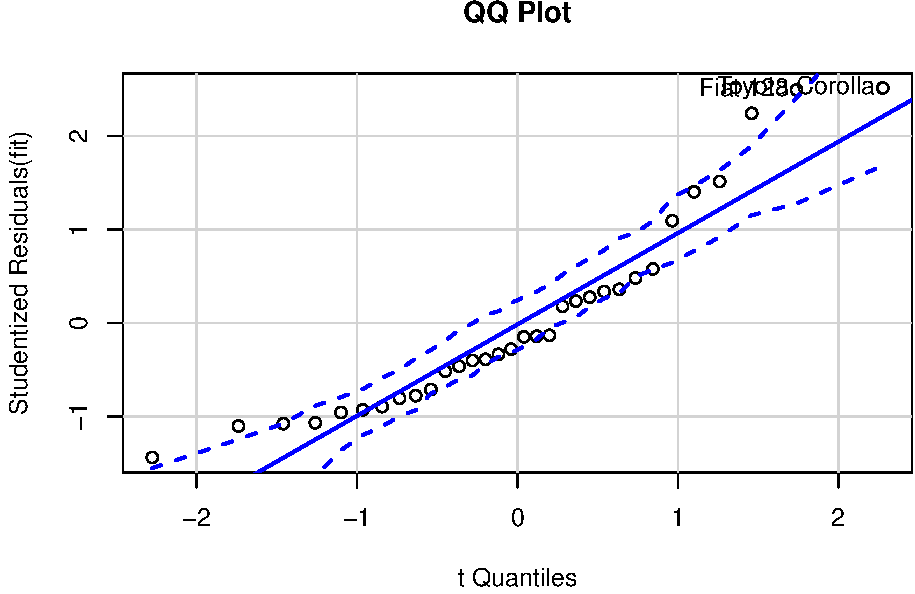
\includegraphics{A03-Regressões_files/figure-latex/Code Block 4-1.pdf}

\begin{verbatim}
##       Fiat 128 Toyota Corolla 
##             18             20
\end{verbatim}

\begin{Shaded}
\begin{Highlighting}[]
\KeywordTok{leveragePlots}\NormalTok{(fit) }\CommentTok{# leverage plots}
\end{Highlighting}
\end{Shaded}

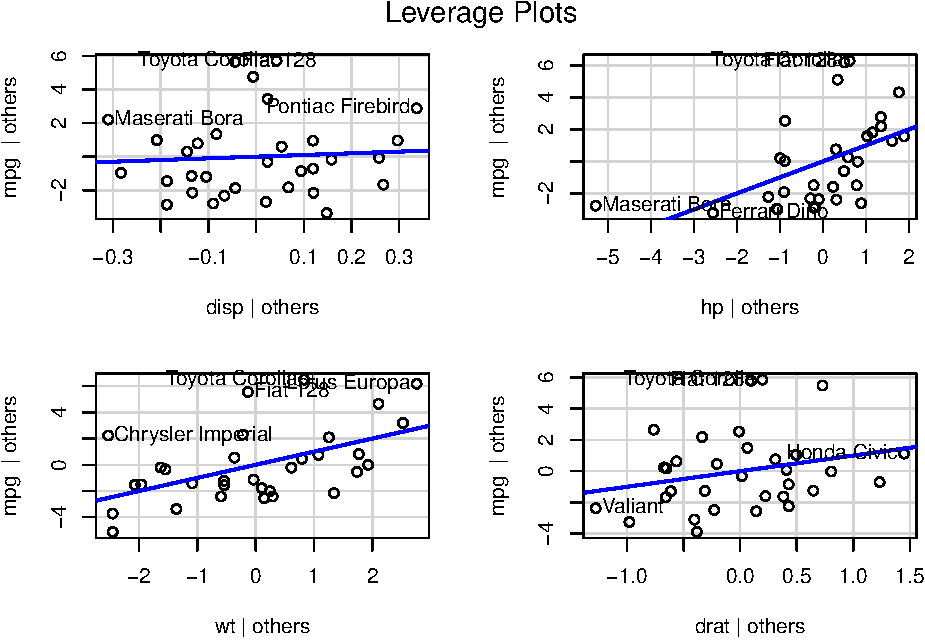
\includegraphics{A03-Regressões_files/figure-latex/Code Block 4-2.pdf}

Avaliando a influência das variáveis\ldots{}

\begin{Shaded}
\begin{Highlighting}[]
\CommentTok{# added variable plots }
\KeywordTok{avPlots}\NormalTok{(fit)}
\end{Highlighting}
\end{Shaded}

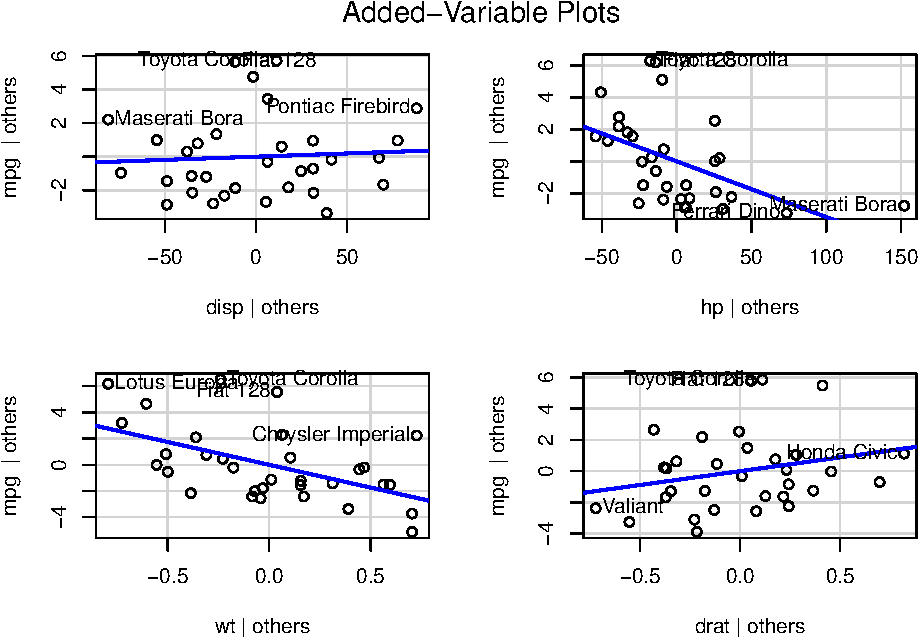
\includegraphics{A03-Regressões_files/figure-latex/Code Block 5-1.pdf}

\begin{Shaded}
\begin{Highlighting}[]
\CommentTok{# Cook's D plot}
\CommentTok{# identify D values > 4/(n-k-1) }
\NormalTok{cutoff <-}\StringTok{ }\DecValTok{4}\OperatorTok{/}\NormalTok{((}\KeywordTok{nrow}\NormalTok{(mtcars)}\OperatorTok{-}\KeywordTok{length}\NormalTok{(fit}\OperatorTok{$}\NormalTok{coefficients)}\OperatorTok{-}\DecValTok{2}\NormalTok{)) }
\KeywordTok{plot}\NormalTok{(fit, }\DataTypeTok{which=}\DecValTok{4}\NormalTok{, }\DataTypeTok{cook.levels=}\NormalTok{cutoff)}
\end{Highlighting}
\end{Shaded}

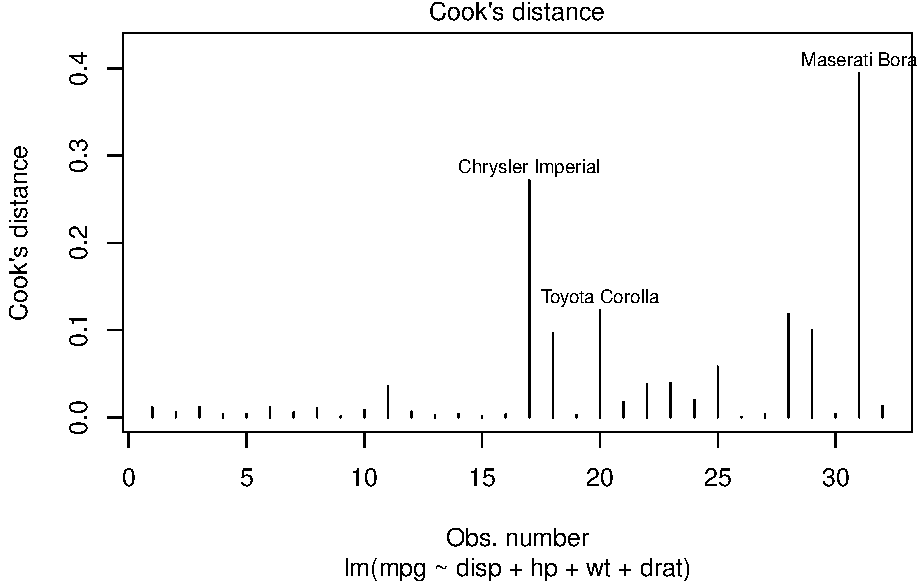
\includegraphics{A03-Regressões_files/figure-latex/Code Block 5-2.pdf}

\begin{Shaded}
\begin{Highlighting}[]
\CommentTok{# Influence Plot }
\KeywordTok{influencePlot}\NormalTok{(fit, }\DataTypeTok{id.method=}\StringTok{"identify"}\NormalTok{, }\DataTypeTok{main=}\StringTok{"Influence Plot"}\NormalTok{, }\DataTypeTok{sub=}\StringTok{"Circle size is proportial to Cook's Distance"}\NormalTok{ )}
\end{Highlighting}
\end{Shaded}

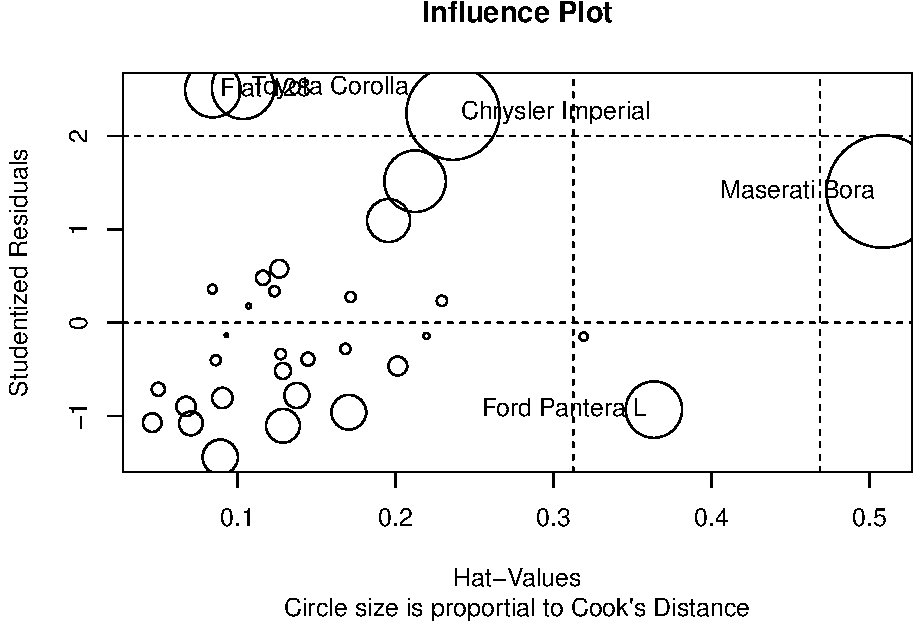
\includegraphics{A03-Regressões_files/figure-latex/Code Block 5-3.pdf}

\begin{verbatim}
##                      StudRes        Hat      CookD
## Chrysler Imperial  2.2446894 0.23636908 0.27133817
## Fiat 128           2.4958292 0.08435766 0.09615527
## Toyota Corolla     2.5159696 0.10355543 0.12213690
## Ford Pantera L    -0.9300234 0.36351495 0.09929551
## Maserati Bora      1.4051504 0.50833966 0.39406393
\end{verbatim}

Avaliando a normalidade dos resíduos\ldots{}

\begin{Shaded}
\begin{Highlighting}[]
\CommentTok{# qq plot for studentized resid}
\KeywordTok{qqPlot}\NormalTok{(fit, }\DataTypeTok{main=}\StringTok{"QQ Plot"}\NormalTok{)}
\end{Highlighting}
\end{Shaded}

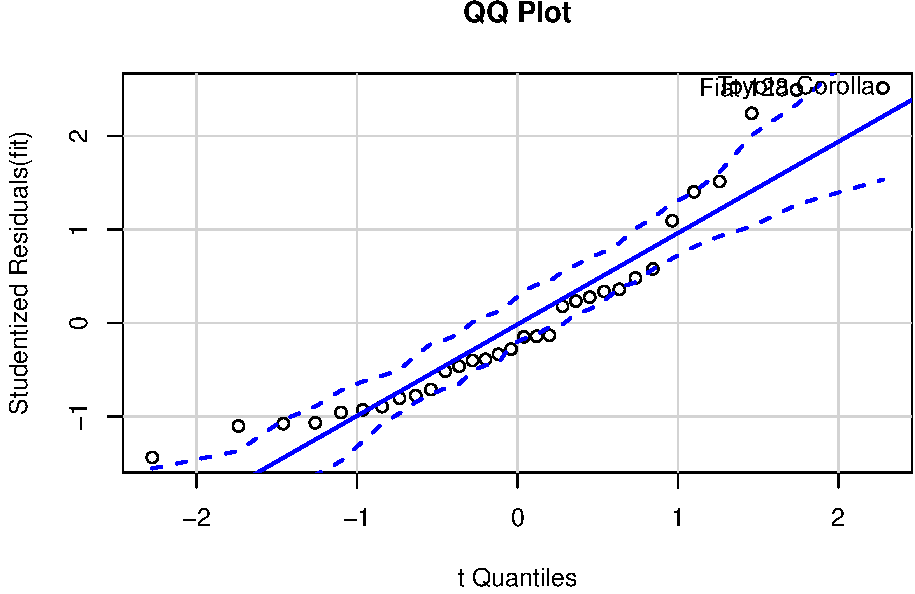
\includegraphics{A03-Regressões_files/figure-latex/Code Block 6-1.pdf}

\begin{verbatim}
##       Fiat 128 Toyota Corolla 
##             18             20
\end{verbatim}

\begin{Shaded}
\begin{Highlighting}[]
\CommentTok{# distribution of studentized residuals}
\KeywordTok{require}\NormalTok{(MASS)}
\NormalTok{sresid <-}\StringTok{ }\KeywordTok{studres}\NormalTok{(fit) }
\KeywordTok{hist}\NormalTok{(sresid, }\DataTypeTok{freq=}\OtherTok{FALSE}\NormalTok{, }
   \DataTypeTok{main=}\StringTok{"Distribution of Studentized Residuals"}\NormalTok{)}
\NormalTok{xfit<-}\KeywordTok{seq}\NormalTok{(}\KeywordTok{min}\NormalTok{(sresid),}\KeywordTok{max}\NormalTok{(sresid),}\DataTypeTok{length=}\DecValTok{40}\NormalTok{) }
\NormalTok{yfit<-}\KeywordTok{dnorm}\NormalTok{(xfit) }
\KeywordTok{lines}\NormalTok{(xfit, yfit)}
\end{Highlighting}
\end{Shaded}

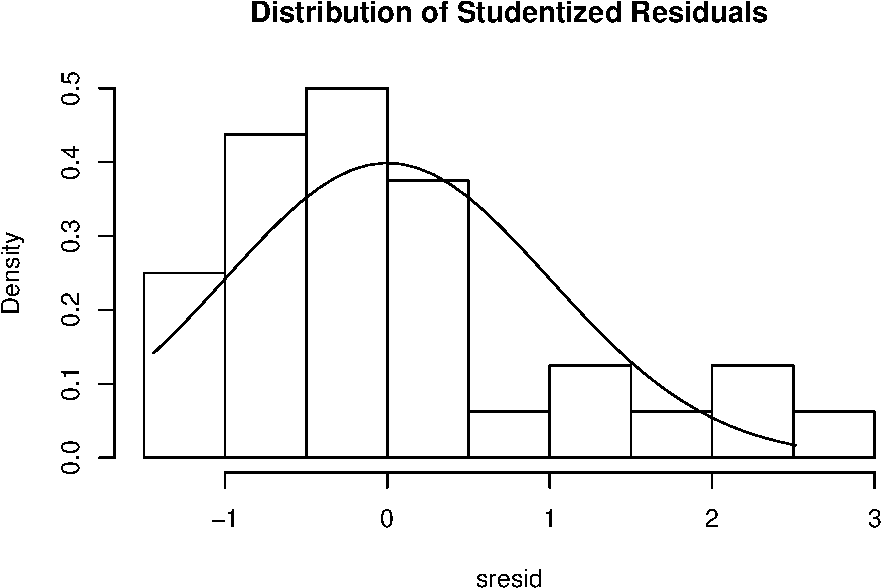
\includegraphics{A03-Regressões_files/figure-latex/Code Block 6-2.pdf}

Avaliando a heterocedasticidade\ldots{}

\begin{Shaded}
\begin{Highlighting}[]
\CommentTok{# non-constant error variance test}
\KeywordTok{ncvTest}\NormalTok{(fit)}
\end{Highlighting}
\end{Shaded}

\begin{verbatim}
## Non-constant Variance Score Test 
## Variance formula: ~ fitted.values 
## Chisquare = 1.429672, Df = 1, p = 0.23182
\end{verbatim}

\begin{Shaded}
\begin{Highlighting}[]
\CommentTok{# plot studentized residuals vs. fitted values }
\KeywordTok{spreadLevelPlot}\NormalTok{(fit)}
\end{Highlighting}
\end{Shaded}

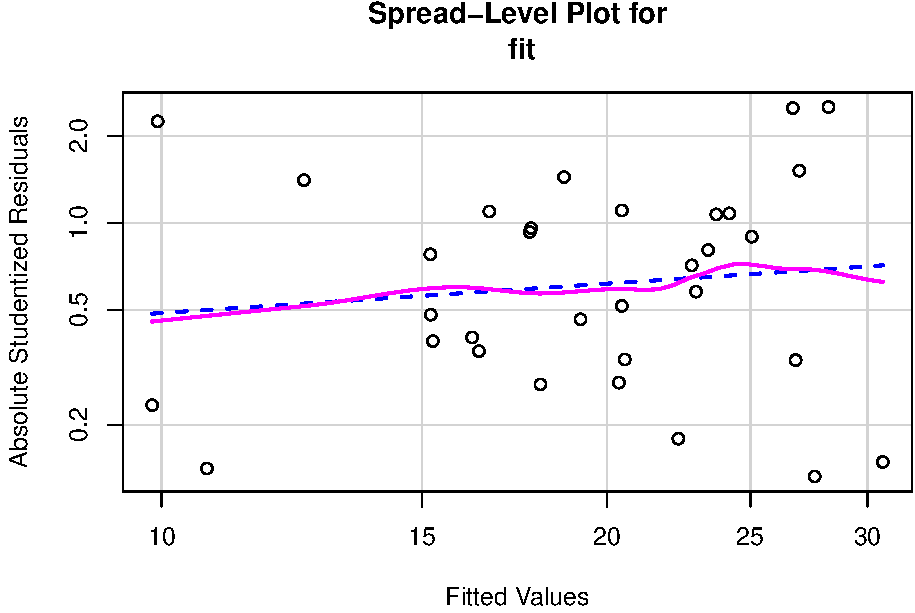
\includegraphics{A03-Regressões_files/figure-latex/Code Block 7-1.pdf}

\begin{verbatim}
## 
## Suggested power transformation:  0.6616338
\end{verbatim}

Avaliando a presença de multicolinearidade\ldots{}

\begin{Shaded}
\begin{Highlighting}[]
\KeywordTok{vif}\NormalTok{(fit) }\CommentTok{# variance inflation factors }
\end{Highlighting}
\end{Shaded}

\begin{verbatim}
##     disp       hp       wt     drat 
## 8.209402 2.894373 5.096601 2.279547
\end{verbatim}

\begin{Shaded}
\begin{Highlighting}[]
\KeywordTok{sqrt}\NormalTok{(}\KeywordTok{vif}\NormalTok{(fit)) }\OperatorTok{>}\StringTok{ }\DecValTok{2} \CommentTok{# problem?}
\end{Highlighting}
\end{Shaded}

\begin{verbatim}
##  disp    hp    wt  drat 
##  TRUE FALSE  TRUE FALSE
\end{verbatim}

Avaliando a independência dos residuos - Erros não
autocorrelacionados\ldots{}

\begin{Shaded}
\begin{Highlighting}[]
\KeywordTok{durbinWatsonTest}\NormalTok{(fit)}
\end{Highlighting}
\end{Shaded}

\begin{verbatim}
##  lag Autocorrelation D-W Statistic p-value
##    1        0.100862      1.735915    0.25
##  Alternative hypothesis: rho != 0
\end{verbatim}

\hypertarget{comparando-modelos}{%
\subsubsection{Comparando modelos}\label{comparando-modelos}}

Você pode comprar modelos com a função \textbf{anova()}. O seguinte
código verifica o impacto de \textbf{wt} e \textbf{vs} na predição de
\textbf{mpg} em relação a um modelo que utiliza apenas \textbf{hp} como
variável preditora.

\begin{Shaded}
\begin{Highlighting}[]
\CommentTok{# compare models}
\NormalTok{fit2 <-}\StringTok{ }\KeywordTok{lm}\NormalTok{(mpg }\OperatorTok{~}\StringTok{ }\NormalTok{hp, }\DataTypeTok{data=}\NormalTok{mtcars)}
\KeywordTok{anova}\NormalTok{(fit2,fit)}
\end{Highlighting}
\end{Shaded}

\begin{verbatim}
## Analysis of Variance Table
## 
## Model 1: mpg ~ hp
## Model 2: mpg ~ disp + hp + wt + drat
##   Res.Df    RSS Df Sum of Sq      F    Pr(>F)    
## 1     30 447.67                                  
## 2     27 182.84  3    264.84 13.036 1.885e-05 ***
## ---
## Signif. codes:  0 '***' 0.001 '**' 0.01 '*' 0.05 '.' 0.1 ' ' 1
\end{verbatim}

\hypertarget{seleuxe7uxe3o-de-variuxe1veis}{%
\subsubsection{Seleção de
Variáveis}\label{seleuxe7uxe3o-de-variuxe1veis}}

A seleção de um subconjunto de variáveis preditoras de um conjunto maior
(por exemplo, seleção por etapas) é um tópico controverso. Você pode
executar a seleção passo a passo (avançar, retroceder, ambos) usando a
função \textbf{stepAIC()} do pacote \textbf{MASS}. O \textbf{stepAIC()}
realiza a seleção do modelo passo a passo pelo AIC exato.

\begin{Shaded}
\begin{Highlighting}[]
\CommentTok{# Stepwise Regression}
\KeywordTok{require}\NormalTok{(MASS)}
\NormalTok{fit <-}\StringTok{ }\KeywordTok{lm}\NormalTok{(mpg }\OperatorTok{~}\StringTok{ }\NormalTok{disp }\OperatorTok{+}\StringTok{ }\NormalTok{hp }\OperatorTok{+}\StringTok{ }\NormalTok{drat }\OperatorTok{+}\StringTok{ }\NormalTok{wt }\OperatorTok{+}\StringTok{ }\NormalTok{qsec }\OperatorTok{+}\StringTok{ }\NormalTok{vs, }\DataTypeTok{data=}\NormalTok{mtcars)}
\NormalTok{step <-}\StringTok{ }\KeywordTok{stepAIC}\NormalTok{(fit, }\DataTypeTok{direction=}\StringTok{"both"}\NormalTok{)}
\end{Highlighting}
\end{Shaded}

\begin{verbatim}
## Start:  AIC=67.42
## mpg ~ disp + hp + drat + wt + qsec + vs
## 
##        Df Sum of Sq    RSS    AIC
## - vs    1     0.224 170.13 65.466
## - disp  1     4.178 174.08 66.201
## - qsec  1     5.760 175.66 66.491
## <none>              169.91 67.424
## - hp    1    12.051 181.96 67.617
## - drat  1    14.800 184.71 68.097
## - wt    1    75.423 245.33 77.180
## 
## Step:  AIC=65.47
## mpg ~ disp + hp + drat + wt + qsec
## 
##        Df Sum of Sq    RSS    AIC
## - disp  1     3.974 174.10 64.205
## <none>              170.13 65.466
## - hp    1    11.886 182.01 65.627
## - qsec  1    12.708 182.84 65.772
## - drat  1    15.506 185.63 66.258
## + vs    1     0.224 169.91 67.424
## - wt    1    81.394 251.52 75.978
## 
## Step:  AIC=64.21
## mpg ~ hp + drat + wt + qsec
## 
##        Df Sum of Sq    RSS    AIC
## - hp    1     9.418 183.52 63.891
## - qsec  1     9.578 183.68 63.919
## <none>              174.10 64.205
## - drat  1    11.956 186.06 64.331
## + disp  1     3.974 170.13 65.466
## + vs    1     0.021 174.08 66.201
## - wt    1   113.882 287.99 78.310
## 
## Step:  AIC=63.89
## mpg ~ drat + wt + qsec
## 
##        Df Sum of Sq    RSS    AIC
## <none>              183.52 63.891
## - drat  1    11.942 195.46 63.908
## + hp    1     9.418 174.10 64.205
## + disp  1     1.506 182.02 65.627
## + vs    1     0.147 183.37 65.865
## - qsec  1    85.720 269.24 74.156
## - wt    1   275.686 459.21 91.241
\end{verbatim}

\begin{Shaded}
\begin{Highlighting}[]
\NormalTok{step}\OperatorTok{$}\NormalTok{anova }\CommentTok{# display results}
\end{Highlighting}
\end{Shaded}

\begin{verbatim}
## Stepwise Model Path 
## Analysis of Deviance Table
## 
## Initial Model:
## mpg ~ disp + hp + drat + wt + qsec + vs
## 
## Final Model:
## mpg ~ drat + wt + qsec
## 
## 
##     Step Df  Deviance Resid. Df Resid. Dev      AIC
## 1                            25   169.9049 67.42409
## 2   - vs  1 0.2242432        26   170.1291 65.46630
## 3 - disp  1 3.9743508        27   174.1035 64.20525
## 4   - hp  1 9.4180913        28   183.5216 63.89108
\end{verbatim}

Como alternativa, você pode executar a regressão de todos os
subconjuntos usando a função \textbf{leaps()} do pacote \textbf{leaps}.
No código a seguir, o \textbf{nbest} indica o número de subconjuntos de
cada tamanho a serem relatados. Aqui, os dez melhores modelos serão
relatados para cada tamanho de subconjunto (1 preditor, 2 preditores
etc.). Copie e cole o código no Console do R para verificar os
resultados.

\begin{Shaded}
\begin{Highlighting}[]
\CommentTok{# All Subsets Regression}
\KeywordTok{require}\NormalTok{(leaps)}
\NormalTok{leaps<-}\KeywordTok{regsubsets}\NormalTok{(mpg }\OperatorTok{~}\StringTok{ }\NormalTok{disp }\OperatorTok{+}\StringTok{ }\NormalTok{hp }\OperatorTok{+}\StringTok{ }\NormalTok{drat }\OperatorTok{+}\StringTok{ }\NormalTok{wt }\OperatorTok{+}\StringTok{ }\NormalTok{qsec }\OperatorTok{+}\StringTok{ }\NormalTok{vs, }\DataTypeTok{data=}\NormalTok{mtcars,}\DataTypeTok{nbest=}\DecValTok{10}\NormalTok{)}
\CommentTok{# view results }
\KeywordTok{summary}\NormalTok{(leaps)}
\CommentTok{# plot a table of models showing variables in each model.}
\CommentTok{# models are ordered by the selection statistic.}
\KeywordTok{plot}\NormalTok{(leaps,}\DataTypeTok{scale=}\StringTok{"r2"}\NormalTok{)}
\CommentTok{# plot statistic by subset size }
\KeywordTok{require}\NormalTok{(car)}
\KeywordTok{subsets}\NormalTok{(leaps, }\DataTypeTok{statistic=}\StringTok{"rsq"}\NormalTok{)}
\end{Highlighting}
\end{Shaded}

\hypertarget{indo-aluxe9m}{%
\subsection{Indo além\ldots{}}\label{indo-aluxe9m}}

O pacote \textbf{relaimpo} fornece medidas de importância relativa para
cada um dos preditores no modelo. Consulte \textbf{help(calc.relimp)}
para obter detalhes sobre as quatro medidas de importância relativa
fornecidas.

\end{document}
